\section{Wikidata Processing}
\label{sec:apdx_wikidata_proc}
We normalize each label by removing parenthetical qualifiers, lowercasing for deduplication, and retaining only short alphabetic or hyphenated terms with at most five words. We further require a non-empty short description from the glossary index that does not simply repeat the term, which filters out many ambiguous or non-English labels. To avoid a corpus dominated by very frequent instance types such as people, taxa, or scholarly articles, we assign each entity a primary \texttt{P31} type using its least frequent instance type and rank terms with inverse-type-frequency sampling. Terms appearing in the held-out evaluation glossaries are removed before training.

For each retained term, we prompt Gemini-2.5-Flash to generate three natural utterances of 5--15 words containing the term (Figure \ref{fig:wikidata_utt_gen}). We then synthesize the utterances with CosyVoice 3\footnote{\url{https://huggingface.co/FunAudioLLM/Fun-CosyVoice3-0.5B-2512}}, using speaker prompts randomly sampled from GigaSpeech.



\section{Speech LLM Data Synthesis}
\label{sec:speechllm_data_synth}

As in InfiniSST, we build robust segments of 28.8 seconds, filter out those with WER larger than 0.1 using parakeet-0.6b-tdt-v2\footnote{\url{https://huggingface.co/nvidia/parakeet-tdt-0.6b-v2}} and generate the target language translation with Qwen3-30B-A3B-Instruct-2507-FP8~\citep{yang2025qwen3technicalreport}\footnote{\url{https://huggingface.co/Qwen/Qwen3-30B-A3B-Instruct-2507-FP8}} and filter out those with MetricX score~\citep{juraska-etal-2024-metricx}\footnote{\url{https://huggingface.co/google/metricx-24-hybrid-xl-v2p6}} worse than -3. Finally we build the interleaved training data using SimAlign~\citep{jalili-sabet-etal-2020-simalign} with LaBSE~\citep{feng-etal-2022-language}. 

\begin{tcolorbox}[
    colback=gray!5,
    colframe=gray!50,
    title=Translation Prompt,
    fonttitle=\bfseries,
    boxrule=0.5pt
]
\ttfamily\small
You are given English document split into lines. Translate each line into Chinese. Do not include any other text.\\
\textless begin\textgreater\\
\{\}\\
\textless end\textgreater
\end{tcolorbox}

\section{Term Duration Distribution}
\label{app:term_duration}
We show the distribution of term duration on GigaSpeech training set in Figure \ref{fig:term_duration}.

\begin{figure}[t]
    \centering
    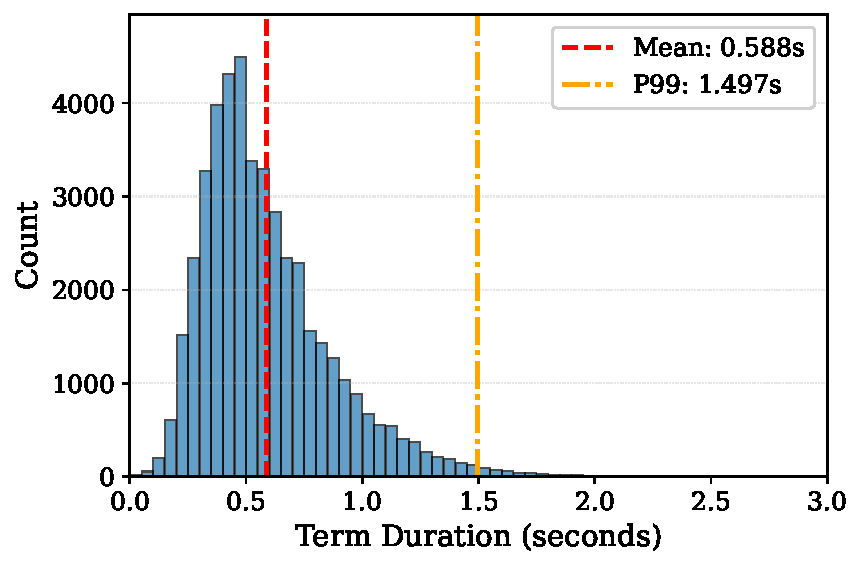
\includegraphics[width=0.9\linewidth]{latex/figures/term_duration_dist.pdf}
    \caption{The distribution of term duration on GigaSpeech training set. }
    \label{fig:term_duration}
\end{figure}

\begin{figure}[t]
\centering

\includegraphics[width=\linewidth]{latex/figures/medicine_main_result.pdf}
\caption{Quality--latency trade-off on ESO dataset En-De direction. Terminology accuracy uses strict exact-form matching. \method improves terminology accuracy and BLEU but not XCOMET.}
\label{fig:eso_de_main}
\end{figure}

\definecolor{trainframe}{RGB}{78, 86, 96}
\definecolor{trainsystembg}{RGB}{245, 248, 252}
\definecolor{trainuserbg}{RGB}{247, 250, 246}
\definecolor{trainassistantbg}{RGB}{255, 249, 239}
\providecommand{\appzh}[1]{\begin{CJK*}{UTF8}{gbsn}#1\end{CJK*}}
\newcommand{\trainbox}[2]{%
    \fcolorbox{trainframe}{#1}{%
        \begin{minipage}{\dimexpr\linewidth-2\fboxsep-2\fboxrule\relax}
        #2
        \end{minipage}%
    }%
}


\begin{figure}[t]
\centering
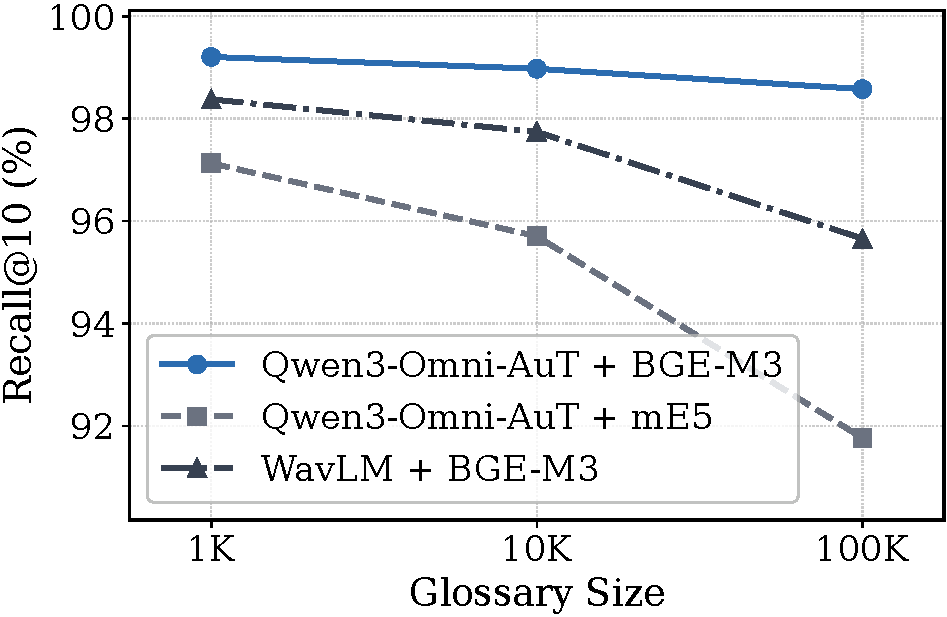
\includegraphics[width=0.8\linewidth]{latex/figures/retriever_encoder_ablation_devraw.pdf}
\caption{Recall@10 across glossary sizes for different encoder combinations. Qwen3-Omni-AuT + BGE-M3 achieves the highest recall.}
\label{fig:ablation_retriever_encoder}
\end{figure}




\begin{figure}[t]
    \centering
    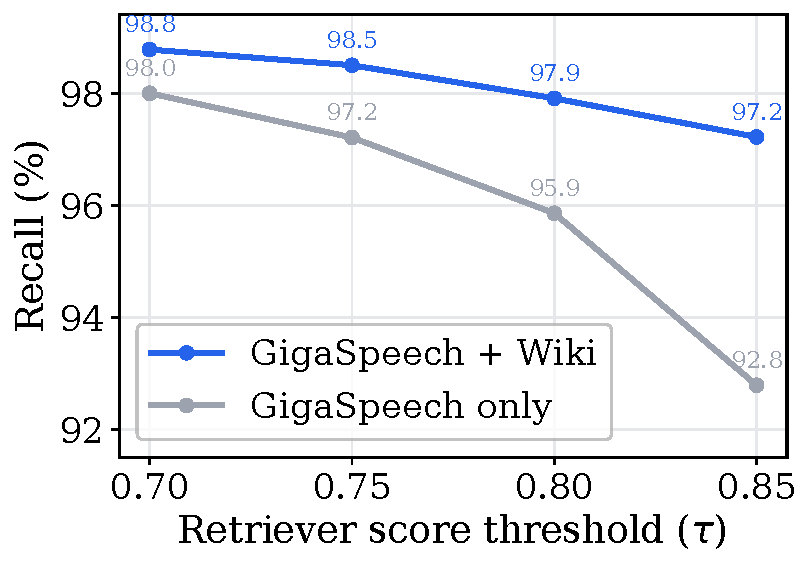
\includegraphics[width=0.8\linewidth]{latex/figures/retriever_data_ablation_dev.pdf}
    \caption{Recall@10 under different threshold $\tau$ on the GigaSpeech dev set for retrievers trained with and without Wikidata.}
    \label{fig:retriever_data}
\end{figure}

\begin{table}[t]
\centering
\setlength{\tabcolsep}{4pt}
\begin{tabular}{lccc}
\toprule
Context Length & 1K & 10K & 100K \\
\midrule
Fixed 1.92s & 98.11 & 97.47 & 95.18 \\
Fixed 3.84s & 98.65 & 98.31 & 97.58 \\
Fixed 5.76s & \textbf{99.64} & \textbf{99.58} & \textbf{99.33} \\
Variable 2.88--5.76s & 99.20 & 98.97 & 98.58 \\
\bottomrule
\end{tabular}
\caption{Recall@10 of retrievers trained with different context lengths, across glossary sizes. Longer speech contexts yield higher recall.}
\label{tab:ablation_context}
\end{table}



\section{Training Details}\label{app:training_details}

\paragraph{Retriever}
We train the retriever with LoRA applied to both the speech and text encoders.
For the audio encoder, LoRA is inserted into the query/key/value/output projections and MLP blocks with rank $r{=}32$ and scaling factor $\alpha{=}64$.
For the text encoder, LoRA targets the query/key/value projections with rank $r{=}16$ and $\alpha{=}32$.
We train with a multi-positive InfoNCE objective using a fixed temperature $\gamma{=}0.03$.
We optimize with AdamW (learning rate $1\times10^{-4}$, weight decay 0.01), cosine annealing with 10\% warmup, and gradient clipping (max norm 1.0) under BF16 mixed precision.
Training is performed with Distributed Data Parallel (DDP) on eight RTX A6000 GPUs with a global batch size of 8192.

\paragraph{Speech LLM}
We fine-tune the Speech LLM using LoRA with rank $r{=}32$ and $\alpha{=}32$.
For Speech LLM training, we enable sequence packing with a maximum packed sequence length of 3,072 tokens and use a global batch size of 4 packed sequences.
We optimize with AdamW (learning rate $1\times10^{-4}$, weight decay 0.01) and gradient clipping (max norm 1.0).
Training is performed with DDP and expert parallelism (EP) of size 2 on four NVIDIA RTX A6000 GPUs.

% \section{Case Study}
% \begin{CJK*}{UTF8}{gbsn}
% \label{sec:case_study}

% We summarize five talks under a fixed chunk size of 1.92 seconds (stride size 0.48 seconds) for En$\rightarrow$Zh translation with ACL glossaries.
% We compare our retrieval-augmented system (RASST) against a baseline without retrieval.
% We compare the average performance across the five sampled talks. 
% As shown in the analysis, \textbf{RASST} achieves an average Term Accuracy of \textbf{0.8930} and a BLEU score of \textbf{47.50}. 
% In contrast, the \textit{baseline} only reaches 0.7299 in Term Accuracy and 45.66 in BLEU. 
% This significant margin demonstrates that RASST consistently preserves key information better than the baseline.

% \paragraph{Chunks with terms.}
% We group term-emission chunks into:
% \begin{itemize}
%   \item \textbf{Category 1 (retrieval correct, RASST correct, base wrong).}
%   Retrieval surfaces the correct glossary entry and RASST realizes it, while the baseline omits or paraphrases it.
%   A representative example is \texttt{2022.acl-long.117} where retrieval includes \texttt{CDA$\rightarrow$CDA} and RASST outputs ``CDA'', but the baseline outputs ``CDR'' (confusion between close acronyms).

%   \item \textbf{Category 2 (retrieval correct, RASST wrong, base correct/wrong).}
%   Retrieval is correct, but RASST fails to realize the glossary surface form.
%   For example in \texttt{2022.acl-long.110}, retrieval includes \texttt{FLR$\rightarrow$最终延迟减少}, yet RASST emits ``FLR'' without the Chinese glossary surface form.

%   \item \textbf{Category 3 (retrieval wrong).}
%   Retrieval fails to include the corresponding glossary entry in the final map at the term-emission chunk.
%   These are term-bearing chunks where the retriever returns an incorrect term list (often topical but irrelevant), and the needed entry is absent.
%   For example, in \texttt{2022.acl-long.117} the chunk requires \textit{baseline}$\rightarrow$基线, but the retrieved map contains unrelated items such as \texttt{data augmentation$\rightarrow$数据增强} and \texttt{domain generalization$\rightarrow$领域泛化} while missing \texttt{baseline$\rightarrow$基线}.
% \end{itemize}

% \paragraph{Chunks without terms.}
% We observe cases where retrieval over-triggers and injects a glossary translation absent from the reference, while the baseline remains consistent with the reference.
% For example, in \texttt{2022.acl-long.110}, RASST emits ``延迟降低'' (from \textit{latency reduction}) whereas the baseline uses ``延迟减少'' (reference-consistent paraphrase).
% \end{CJK*}

\section{Additional Ablations}
\label{sec:apdx_ablation}

This section reports additional ablations that do not fit in the main text.

\begin{figure*}[t]
\centering
% Dev-only tau-selection evidence: fixed raw denominator over raw/10k/100k banks.
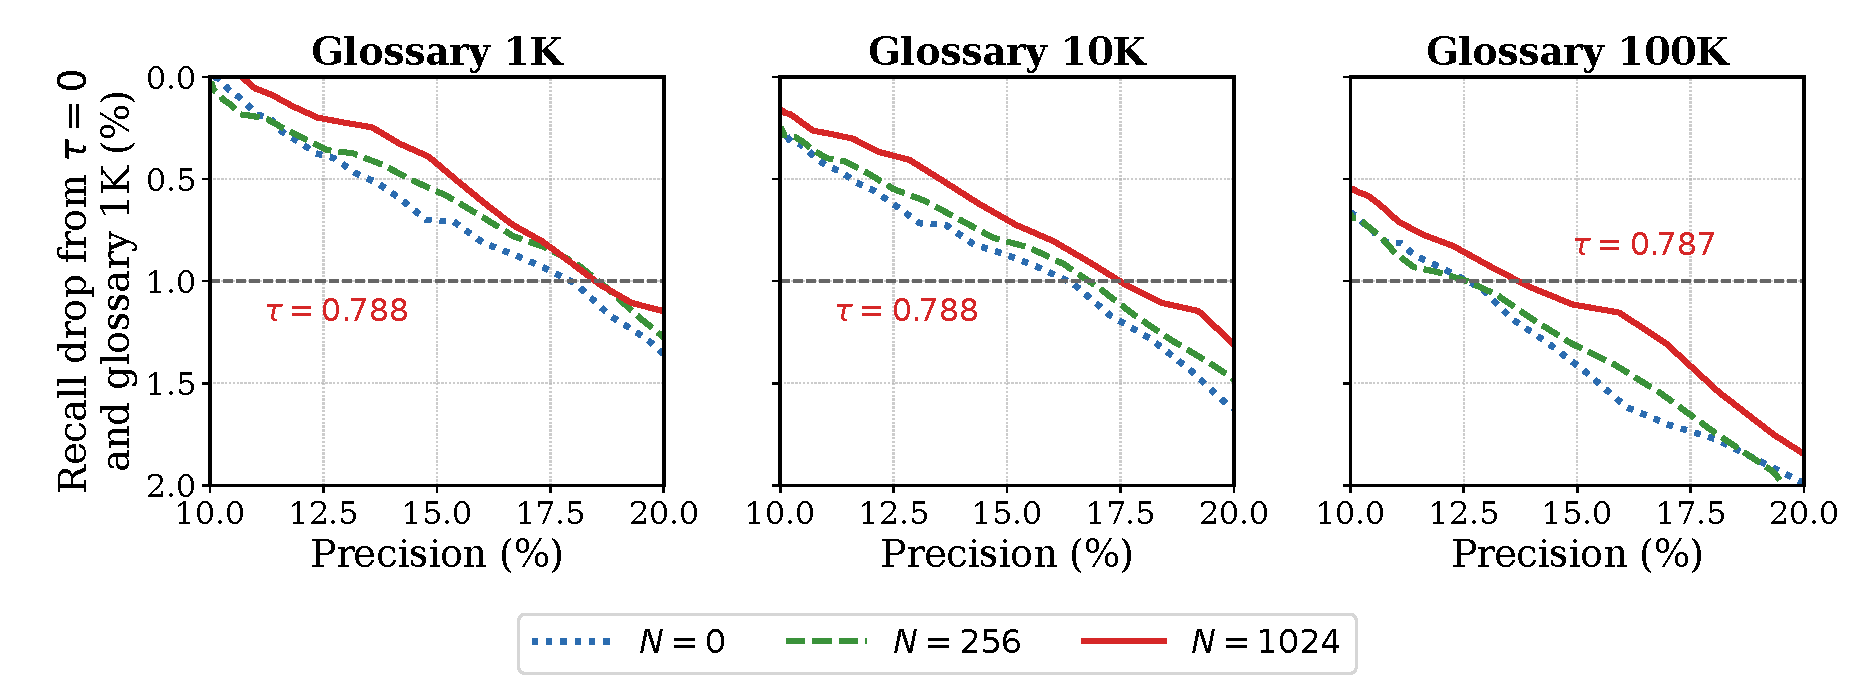
\includegraphics[width=0.9\linewidth]{latex/figures/retriever_dev_pr_fixedraw_hn_comparison.pdf}
\caption{Precision--recall curves across glossary sizes for retrievers trained with $N{=}0, 256, 1024$ hard negatives, obtained by sweeping $\tau \in [0,1]$. The dashed horizontal line marks a 1\% recall drop; the red annotations show the corresponding $\tau\approx0.78$ operating points.}
\label{fig:ablation_hn_tau}
\end{figure*}


\begin{figure*}
    \centering
    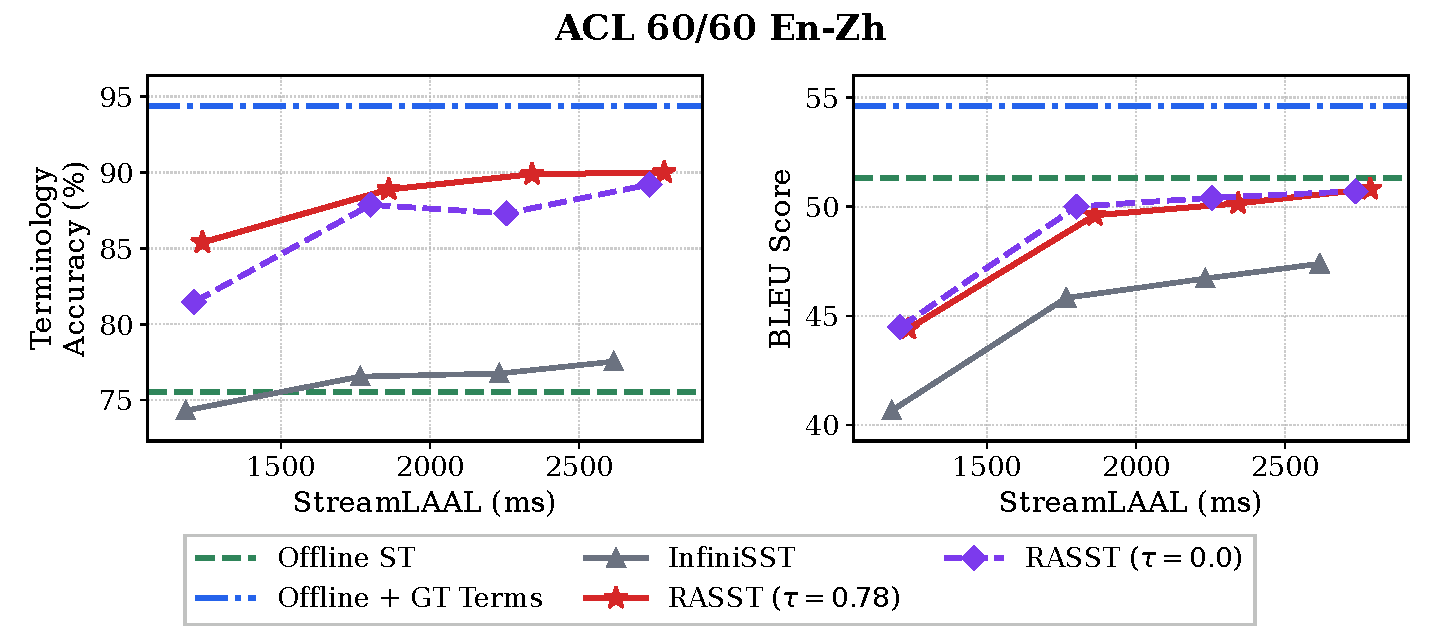
\includegraphics[width=0.9\linewidth]{latex/figures/speechllm_ablation_zh_tau_compare.pdf}
    \caption{Quality–latency trade-off of \method with $\tau=0$ and $\tau=0.78$.} 
    \label{fig:ablation_speechllm_tau}
\end{figure*}



\paragraph{Retriever training data} 
We examine the impact of training data by comparing our default retriever, trained on both GigaSpeech and Wikidata, against a GigaSpeech-only variant. As shown in Figure~\ref{fig:retriever_data}, adding Wikidata substantially improves recall, with the largest gains at high $\tau$, indicating that the retriever assigns higher similarity to true positives when trained with Wikidata.

\paragraph{Retriever encoders}
 We test different encoder combinations here. We additionally tried mE5 text encoder~\citep{wang2024multilingual}\footnote{\url{https://huggingface.co/intfloat/multilingual-e5-large}} and WavLM-large speech encoder~\citep{wavlm}\footnote{\url{https://huggingface.co/microsoft/wavlm-large}}. As shown in Figure~\ref{fig:ablation_retriever_encoder}, Qwen3-Omni Audio Transformer + BGE-M3 achieves the best recall.

\paragraph{Retriever context length.}
\method trains the retriever with variable-length speech contexts and here we compare against fixed-length alternatives. As shown in Table~\ref{tab:ablation_context}, longer fixed-length contexts generally yield higher recall across glossary sizes. The variable-length setup matches the recall of the longest fixed-length context (5.76s) while offering better flexibility at inference.

\paragraph{Term-Tag Supervision}
The \texttt{\textless term\textgreater} tags in Speech LLM targets explicitly identify when a retrieved translation is realized. We train an otherwise matched En--Zh model without these tags. As shown in Figure~\ref{fig:term_tag_ablation}, the tagged model improves exact-form TERM\_ACC by 3.60--5.06 points across all latency settings while achieving similar BLEU scores, supporting the use of tags as training-time supervision. The tags are stripped before evaluation and are not displayed to user. 

\begin{figure}[t]
\centering
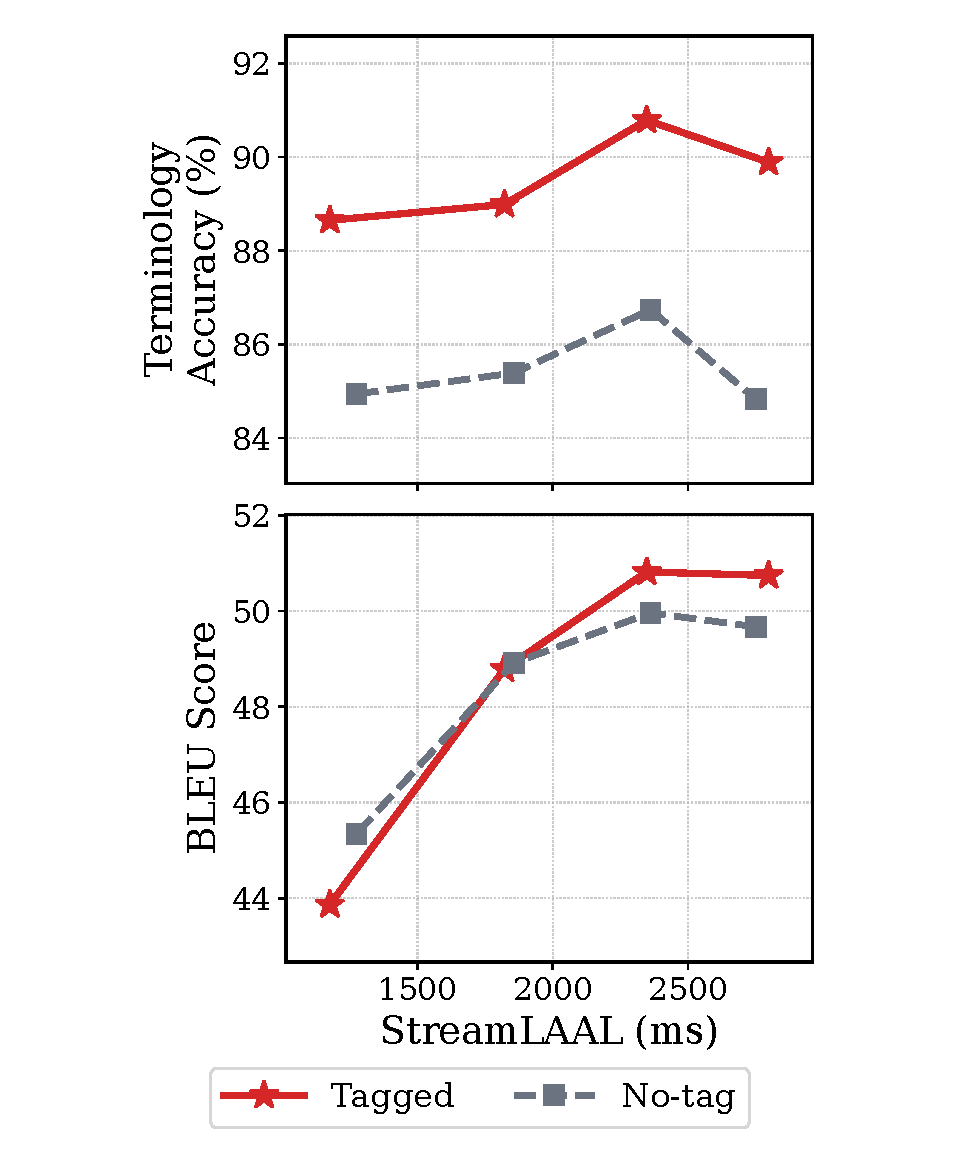
\includegraphics[width=\linewidth]{latex/figures/term_tag_ablation.pdf}
\caption{En--Zh ablation of training-time term tags. LAAL is in milliseconds and TERM is exact-form TERM\_ACC (\%).}
\label{fig:term_tag_ablation}
\end{figure}

\begin{figure*}[t]
\centering
\begingroup
\setlength{\fboxsep}{5pt}
\setlength{\fboxrule}{0.35pt}
\renewcommand{\arraystretch}{1.08}
\scriptsize
\begin{tabularx}{\textwidth}{@{}>{\bfseries}p{0.12\textwidth}>{\raggedright\arraybackslash}X@{}}
System & \trainbox{trainsystembg}{You are a professional simultaneous interpreter. You will be given chunks of English audio and you need to translate the audio into Chinese text. Use the \texttt{term\_map} as a reference for terminology if provided.} \\
\addlinespace[0.45ex]
User 1 & \trainbox{trainuserbg}{\texttt{<audio>} \par \textbf{term\_map:} \texttt{things} $\rightarrow$ \appzh{事}; \texttt{everything} $\rightarrow$ \appzh{所有努力}; \texttt{right} $\rightarrow$ \appzh{权利}; \texttt{thing} $\rightarrow$ \appzh{东西}; \texttt{that thing} $\rightarrow$ \appzh{那东西}.} \\
Assistant 1 & \trainbox{trainassistantbg}{\appzh{她会做些我本意不想让她做的}\texttt{<term>}\appzh{事}\texttt{</term>}\appzh{。这样一来，之前}\texttt{<term>}\appzh{所有努力}\texttt{</term>}\appzh{都白费了，我不得不重新写一遍。}} \\
\addlinespace[0.45ex]
User 2 & \trainbox{trainuserbg}{\texttt{<audio>} \par \textbf{term\_map:} \texttt{the Porch Gable} $\rightarrow$ \appzh{门廊小屋}; \texttt{story} $\rightarrow$ \appzh{传说}; \texttt{Anne} $\rightarrow$ \appzh{安妮}; \texttt{seclusion} $\rightarrow$ \appzh{静谧}; \texttt{Diana} $\rightarrow$ \appzh{戴安娜}; \texttt{gabelle} $\rightarrow$ \appzh{法国盐税}; \texttt{that story} $\rightarrow$ \appzh{这个故事}; \texttt{porch} $\rightarrow$ \appzh{门廊}.} \\
Assistant 2 & \trainbox{trainassistantbg}{\appzh{然而，最终}\texttt{<term>}\appzh{传说}\texttt{</term>}\appzh{终于完成了，}\texttt{<term>}\appzh{安妮}\texttt{</term>}\appzh{在}\texttt{<term>}\appzh{门廊小屋}\texttt{</term>}\appzh{的}\texttt{<term>}\appzh{静谧}\texttt{</term>}\appzh{中把它读给了}\texttt{<term>}\appzh{戴安娜}\texttt{</term>}\appzh{听。她}} \\
\addlinespace[0.45ex]
User 3 & \trainbox{trainuserbg}{\texttt{<audio>} \par \textbf{term\_map:} \texttt{Diana} $\rightarrow$ \appzh{戴安娜}; \texttt{watchful eye} $\rightarrow$ \appzh{密切留意}; \texttt{Robert Ray} $\rightarrow$ \appzh{罗伯特·雷}; \texttt{her pathetic scene} $\rightarrow$ \appzh{那个悲情场景}; \texttt{scene} $\rightarrow$ \appzh{现场}; \texttt{that scene} $\rightarrow$ \appzh{那场戏}.} \\
Assistant 3 & \trainbox{trainassistantbg}{\appzh{成功地呈现了那个悲情场景，同时又没有牺牲}\texttt{<term>}\appzh{罗伯特·雷}\texttt{</term>}\appzh{，她一边读一边}\texttt{<term>}\appzh{密切留意}\texttt{</term>}\appzh{着}\texttt{<term>}\appzh{戴安娜}\texttt{</term>}\appzh{的反应。戴安娜}} \\
\end{tabularx}
\endgroup
\caption{An example of En-Zh Speech LLM training data.}
\label{fig:train_prompt_visual}
\end{figure*}

\section{\texorpdfstring{Form-Aware Terminology Accuracy}{Form-Aware Terminology Accuracy}}
\label{app:form_aware_metric}


The primary exact-form scorer first segments system hypothesis into sentences each aligned to a reference sentence. A glossary entry is eligible when its English source form occurs in the aligned source sentence and its target form occurs in the reference. Target forms are deduplicated, and each eligible target form is counted once per sentence. Form-aware metrics uses the same setting as exact-form scorer and differs only in determining whether the target form appears in the hypothesis sentence.

For reproducibility, let $N(z)$ denote Unicode NFKC normalization followed by case folding and whitespace collapse. Let $C(z)$ concatenate only the Unicode letters and numbers in $N(z)$, thereby removing spaces, punctuation, and hyphens. For every eligible target form $t$ and aligned hypothesis $h$, we apply the following ordered rules; the first successful rule determines the match type.
\begin{enumerate}[leftmargin=*,nosep]
    \item \textbf{Exact form.} Accept if the unnormalized glossary target $t$ is a substring of the unnormalized hypothesis $h$.
    \item \textbf{Normalized surface form.} If $t$ consists only of Latin letters or digits and $|C(t)|<4$, accept only when $N(t)$ occurs in $N(h)$ with Unicode word boundaries on both sides. For every other target, accept when $N(t)$ is a substring of $N(h)$. This rule handles case and Unicode-width variation without allowing a short acronym to match inside a longer word.
    \item \textbf{Spacing or hyphenation variant.} If the previous rules fail, accept when $C(t)$ is a substring of $C(h)$, provided that $|C(t)|\geq4$ for Latin-alphanumeric targets and $|C(t)|\geq2$ otherwise. The minimum lengths prevent permissive matches for very short strings.
    \item \textbf{German inflection.} For En--De only, if the previous rules fail, tokenize $t$ and $h$, discard punctuation and whitespace tokens, normalize each lemma with $N(\cdot)$, and accept only if the complete lemma sequence of $t$ equals a contiguous subsequence of the lemma sequence of $h$. We use spaCy 3.8.5 with \texttt{de\_core\_news\_sm} 3.8.0 and disable its parser and named-entity recognizer.
\end{enumerate}
The form-aware score counts a term as correct if any rule succeeds. It never accepts a synonym, paraphrase, reordered lemma sequence, or merely semantically related expression. Normalization is used only to test the hypothesis; eligibility continues to require the prescribed target surface form in the reference. The diagnostic was run on existing hypotheses, not newly decoded outputs. Across 32 system settings, it scored 27,296 eligible occurrences; every row with archived exact numerator and denominator reproduced the original exact count.


\begin{table}[t]
\centering
% \color{red}
% \scriptsize
\setlength{\tabcolsep}{3pt}
\begin{tabular}{lrrr}
\toprule
Condition & Exact & Form-aware & $\Delta$ \\
\midrule
ACL En--Zh & 88.99 & 89.10 & +0.11 \\
ACL En--Ja & 84.57 & 84.57 & +0.00 \\
ACL En--De & 82.99 & 87.38 & +4.39 \\
ESO En--De & 78.21 & 82.23 & +4.02 \\
\bottomrule
\end{tabular}
\caption{RASST exact-form and conservative form-aware TERM\_ACC (\%) at latency multiplier 2.}
\label{tab:form_aware}
\end{table}


As shown in Table \ref{tab:form_aware}, the largest adjustment is in German, where inflection and productive compounding create valid surface variants. At latency multiplier 2, ACL En--De InfiniSST also rises from 67.59 to 74.44, while \method rises from 82.99 to 87.38; the form-aware margin therefore remains 12.94 points. On ESO En--De the corresponding margin is 23.03 points (82.23 versus 59.20). Thus normalization reduces both systems' apparent error, without changing the conclusion that retrieval improves terminology realization.


% \begin{table*}[t]
% \centering
% \color{red}
% \scriptsize
% \setlength{\tabcolsep}{4pt}
% \begin{tabular}{llrrrrr}
% \toprule
% Direction & LM & \method LAAL & \method XCOMET & InfiniSST LAAL & InfiniSST XCOMET & $\Delta$ XCOMET \\
% \midrule
% En--Zh & 1 & 1175.8 & 78.1183 & 1181.1 & 78.0393 & +0.0789 \\
% En--Zh & 2 & 1821.5 & 82.3465 & 1765.7 & 82.2024 & +0.1442 \\
% En--Zh & 3 & 2347.3 & 85.1050 & 2232.7 & 84.1425 & +0.9624 \\
% En--Zh & 4 & 2797.6 & 84.3743 & 2616.3 & 83.0173 & +1.3570 \\
% \midrule
% En--De & 1 & 1026.4 & 82.2508 & 1121.0 & 81.6160 & +0.6347 \\
% En--De & 2 & 1666.9 & 83.7358 & 1759.1 & 84.2266 & -0.4907 \\
% En--De & 3 & 2253.8 & 83.3494 & 2390.0 & 83.2341 & +0.1154 \\
% En--De & 4 & 2756.9 & 82.2060 & 2826.7 & 82.4453 & -0.2393 \\
% \midrule
% En--Ja & 1 & 1477.7 & 59.1527 & 1613.0 & 63.2561 & -4.1034 \\
% En--Ja & 2 & 2231.1 & 70.3791 & 2291.2 & 72.6553 & -2.2762 \\
% En--Ja & 3 & 2777.6 & 75.7851 & 2913.0 & 75.0910 & +0.6941 \\
% En--Ja & 4 & 3212.3 & 77.6470 & 3400.5 & 73.1345 & +4.5125 \\
% \bottomrule
% \end{tabular}
% \caption{\crchange{XCOMET-XXL (multiplied by 100) on ACL 60/60. LAAL is in milliseconds.}}
% \label{tab:acl_xcomet}
% \end{table*}




% \begin{table*}[t]
% \centering
% \color{red}
% \scriptsize
% \setlength{\tabcolsep}{4pt}
% \begin{tabular}{lrrrrrrrr}
% \toprule
% LM & Tagged LAAL & Tagged BLEU & Tagged TERM & No-tag LAAL & No-tag BLEU & No-tag TERM & $\Delta$ BLEU & $\Delta$ TERM \\
% \midrule
% 1 & 1175.8 & 43.8652 & 88.65 & 1274.4 & 45.3446 & 84.94 & -1.4794 & +3.71 \\
% 2 & 1821.5 & 48.7921 & 88.99 & 1857.2 & 48.9172 & 85.39 & -0.1251 & +3.60 \\
% 3 & 2347.3 & 50.8150 & 90.79 & 2361.0 & 49.9595 & 86.74 & +0.8554 & +4.05 \\
% 4 & 2797.6 & 50.7421 & 89.89 & 2749.6 & 49.6701 & 84.83 & +1.0720 & +5.06 \\
% \bottomrule
% \end{tabular}
% \caption{\crchange{En--Zh ablation of training-time term tags. LAAL is in milliseconds and TERM is exact-form TERM\_ACC (\%). Deltas are tagged minus no-tag.}}
% \label{tab:term_tag_ablation}
% \end{table*}

\section{\texorpdfstring{Robustness to Glossary and Retrieval Quality}{Robustness to Glossary and Retrieval Quality}}
\label{sec:robustness_analysis}

\subsection{\texorpdfstring{Paper-Derived Glossaries}{Paper-Derived Glossaries}}

To approximate a less curated setting, we extract a separate glossary from the paper PDF corresponding to each ACL talk using Gemini, without consulting the transcripts, references, or human-annotated glossary. These glossaries overlap with only 57 of 238 human-annotated glossary entries (23.95\% source-term coverage). We use the paper-derived glossary for \method retrieval but retain the human glossary as the fixed TERM\_ACC denominator for both systems. Table~\ref{tab:paper_glossary} shows the latency-multiplier-2 results. As expected, the gains are much smaller because retrieval cannot supply entries absent from the glossary. Nevertheless, terminology accuracy improves for En--Zh and En--De. 

\begin{table}[t]
\centering
% \color{red}
% \scriptsize
\setlength{\tabcolsep}{3pt}
\begin{tabular}{lcc}
\toprule
Direction & TERM ACC & BLEU \\
\midrule
En--Zh & 77.87 / 75.17 & 46.32 / 45.82 \\
En--Ja & 65.32 / 65.96 & 27.76 / 27.72 \\
En--De & 70.91 / 68.21 & 29.20 / 30.27 \\
\bottomrule
\end{tabular}
\caption{ACL latency-multiplier-2 evaluation with paper-derived retrieval glossaries. Cells show \method / InfiniSST.}
\label{tab:paper_glossary}
\end{table}

\subsection{\texorpdfstring{Retrieval Degradation}{Retrieval Degradation}}

We replace 25\% or 50\% of retrieved entries with irrelevant entries from the same ACL glossary, holding the number of hints and inference configuration fixed. Table~\ref{tab:retrieval_degradation} reports results at latency multiplier 2. Exact-form TERM\_ACC decreases by at most 7.59 points under 50\% replacement and remains above the corresponding InfiniSST accuracy in all three directions. All six corrupted settings have lower XCOMET than their language's uncorrupted setting while have similar BLEU.

\begin{table}[t]
\centering
% \color{red}
% \scriptsize
\setlength{\tabcolsep}{2.5pt}
\begin{tabular}{llrrr}
\toprule
Dir. & Replaced & TERM & BLEU & XCOMET \\
\midrule
En--Zh & 0\%  & 90.00 & 47.878 & 83.628 \\
En--Zh & 25\% & 88.09 & 48.137 & 83.028 \\
En--Zh & 50\% & 85.73 & 48.331 & 82.608 \\
\midrule
En--De & 0\%  & 83.10 & 30.869 & 83.966 \\
En--De & 25\% & 79.79 & 31.077 & 83.214 \\
En--De & 50\% & 75.51 & 31.584 & 83.496 \\
\midrule
En--Ja & 0\%  & 84.57 & 29.889 & 70.379 \\
En--Ja & 25\% & 82.77 & 28.717 & 68.417 \\
En--Ja & 50\% & 78.40 & 27.717 & 67.137 \\
\bottomrule
\end{tabular}
\caption{Sensitivity to retrieval quality at latency multiplier 2. We randomly replaced 0, 25\%, 50\% of the retrieved terms with irrelevant terms. Decoding uses temperature 0.6.}
\label{tab:retrieval_degradation}
\end{table}


\section{\texorpdfstring{{Qualitative and Failure Analysis}}{Qualitative and Failure Analysis}}
\label{sec:qualitative_analysis}

At latency multiplier 2, ACL 60/60 contains 3,266 evaluated terminology occurrences across the three directions. \method is exact-match correct in 638 cases where InfiniSST is wrong, while the reverse occurs in 127 cases. We manually categorize these 127 apparent regressions in Table~\ref{tab:qualitative_errors}.

\begin{table}[t]
\centering
% \color{red}
\small
\begin{tabular}{lr}
\toprule
Category & Occurrences \\
\midrule
Synonym & 28 \\
Grammar-conditioned surface change & 3 \\
Spacing or capitalization & 12 \\
StreamLAAL segmentation error & 48 \\
Term absent & 14 \\
Different concept or named entity & 22 \\
\midrule
Total & 127 \\
\bottomrule
\end{tabular}
\caption{Manual categorization of cases where InfiniSST is exact-match correct and \method is not.}
\label{tab:qualitative_errors}
\end{table}

The first three categories contain the intended term but not the reference surface form, for example ``Softmax'' versus ``Soft max'' and ``Transformer'' versus ``transformer.'' They account for 43 cases and motivate the form-aware diagnostic. A further 48 are boundary artifacts from mWERSegmenter splitting Chinese or Japanese output mid-sentence.

Of the 14 genuinely absent terms, seven are not retrieved because their similarity falls just below $\tau{=}0.78$. The other seven are retrieved but not used: some hints arrive near the end of a sentence after the model has started generating another sentence, while others are omitted because the concept is inferable from context. The remaining 22 cases are genuine substitutions or hallucinations, including ``BETO'' rendered as ``BERT.'' Acoustic acronym confusions also occur without retrieval, such as ``BLEU'' rendered as ``blue.''

\FloatBarrier
\section{\texorpdfstring{ESO Glossary Construction}{ESO Glossary Construction}}
\label{app:eso_glossary}

We construct the ESO hard-term glossary with the following seven-stage pipeline. (1) GPT-5.4 processes batches of 10 sentences with full-talk context, extracts high-precision medical candidates, and associates each candidate with exact target spans; the dataset-provided German sentence translation is kept unchanged. (2) GPT-5.4 enforces exact-span and abbreviation consistency, dropping copied or speculative acronyms. (3) Deterministic checks retain only entries whose source and target strings occur in their corresponding sentences. (4) We deduplicate and normalize source forms without changing target strings. (5) GPT-5.4 examines batches of three terms against no-retrieval outputs and identifies terms that are genuinely difficult rather than harmless variants. (6) We manually inspect and correct the glossary. (7) We serialize the final 215 rows (212 unique English terms) used to build the index. Precision is prioritized over recall throughout.

\begin{tcolorbox}[
  colback=black!2,
  colframe=black!55!black,
  coltext=black,
  title={Stage 1 prompt: candidate extraction},
  fonttitle=\bfseries,
  boxrule=0.4pt]
\ttfamily\footnotesize
Given the full transcript and sentence-level JSON, return one JSON item per sentence. Reuse the provided German translation exactly. Extract only genuinely domain-specific concepts such as procedures, diagnoses, biomarkers, clinical-trial terminology, anatomical terms, and acronyms. Exclude generic nouns, people, organizations, and vague phrases. For each retained English term, return a German target that is a contiguous substring of the provided German sentence. Precision is more important than recall; return an empty term list when no sufficiently technical term is present.
\end{tcolorbox}

\begin{tcolorbox}[
  colback=black!2,
  colframe=black!55!black,
  coltext=black,
  title={Stage 2 prompt: exact span and abbreviation consistency},
  fonttitle=\bfseries,
  boxrule=0.4pt]
\ttfamily\footnotesize
Revise each candidate so every kept target is an exact contiguous span of the sentence translation. Do not add new terms. For abbreviations, keep the item only when its expansion or translation is clear and meaningful; drop a copied acronym, a speculative expansion, or an abbreviation that duplicates a full-form term. Preserve sentence and term identifiers and return JSON only.
\end{tcolorbox}

\begin{tcolorbox}[
  colback=black!2,
  colframe=black!55!black,
  coltext=black,
  title={Stage 5 prompt: hard-term filtering},
  fonttitle=\bfseries,
  boxrule=0.4pt]
\ttfamily\footnotesize
Given the English term, prescribed target, source sentence, reference, and no-RAG prediction, judge whether the prediction conveys the term in context. Accept exact forms, faithful synonyms, and harmless spelling or spacing variants. Mark wrong or missing when the term is omitted, mistranslated, over-generalized, replaced by another concept, or merely copied when an expansion is required. Use not assessable only for alignment failure and return one JSON judgment per identifier.
\end{tcolorbox}

\begin{figure*}[t] % 使用 figure* 环境使其跨双栏
\begin{tcolorbox}[
    enhanced,
    % breakable, % 注意：在浮动环境（figure*）中无法跨页，如果你希望它浮动在顶部/底部，通常不需要 breakable
    colback=gray!3,
    colframe=gray!55!black,
    title={Prompt template for Wikidata term utterance generation},
    fonttitle=\bfseries,
    boxrule=0.4pt,
    arc=1mm,
    left=1.5mm,
    right=1.5mm,
    top=1mm,
    bottom=1mm,
    width=\textwidth % 确保宽度撑满双栏
]
{\ttfamily\footnotesize
\textbf{System instruction:}\par
You are a dataset builder for speech recognition research.\par
Your task: given a list of terms with their short descriptions, generate short English utterances (5--15 words each) that a speaker might say in a lecture, tutorial, or technical discussion. Use the description as context to produce accurate, meaningful sentences, but do NOT just copy the description.\par
Each utterance MUST contain the given term EXACTLY as written (same spelling, but case may differ). Vary sentence structure and term position (beginning, middle, end). Do NOT repeat the same pattern across terms.\par
Output valid JSON only -- no markdown fences, no explanation.\par
\vspace{0.5em}
\textbf{User prompt:}\par
Generate \{variants\_per\_term\} short utterances (5--15 words) for EACH of the following terms. Use the description as context to make the utterance accurate and meaningful. Each utterance must contain the term verbatim.\par
\vspace{0.5em}
Terms with descriptions:\par
[\par
\hspace*{1em}\{"term": "Seismology", "description": "scientific study of earthquakes"\},\par
\hspace*{1em}\{"term": "dataflow graph", "description": "graph representation of data dependencies"\}\par
]\par
\vspace{0.5em}
Return a JSON object mapping each term to a list of \{variants\_per\_term\} utterance strings. Example format:\par
\{\par
\hspace*{1em}"Seismology": [\par
\hspace*{2em}"Seismology helps us understand earthquake patterns.",\par
\hspace*{2em}"The field of seismology has advanced rapidly."\par
\hspace*{1em}]\par
\}\par
\vspace{0.5em}
IMPORTANT: output raw JSON only, no markdown code fences.\par
}
\end{tcolorbox}
\caption{Prompt template for Wikidata term utterance generation.}
\label{fig:wikidata_utt_gen}
\end{figure*}
